%-------------------------------------------------------------------------------
%	EMPIEZA CAPITULO
%-------------------------------------------------------------------------------

\chapter{Introducción al control óptimo}

    Sea el sistema descrito por la representación de estado:

    \begin{equation} \label{eq:conop1}
        \frac{dx}{dt} = A x + b u
    \end{equation}

    donde $A \in \mathbb{R}^{n \times n}$, $b \in \mathbb{R}^{n \times n}$, con condiciones iniciales $x(0) = x_0 \in \mathbb{R}^n$; se desea minimizar el indice de desempeño:

    \begin{equation} \label{eq:conop2}
        J(x, u) = \frac{1}{2} \int_0^{\infty} \left( x^T Q x + \rho u^2 \right) dt
    \end{equation}

    donde $\rho > 0$ y $Q = Q^T \ge 0$, a lo largo de las trayectorias solución de la ecuación~\ref{eq:conop1}. Es decir se desea minimizar la ecuación~\ref{eq:conop2} con las restricciones de la ecuación~\ref{eq:conop1}.

    Este problema de minimización con restricciones se va a resolver usando los multiplicadores de Lagrange.

    El indice de desempeño aumentado es:

    \begin{equation*}
        Ja(x, u, \lambda) = \int_0^{\infty} \left( \frac{1}{2}  \left( x^T Q x + \rho u^2 \right) + \lambda^T \left( Ax + bu - \frac{dx}{dt} \right) \right)
    \end{equation*}

    Definiendo los siguientes funcionales:

    \begin{description}
        \item [Lagrangiano]
        \begin{equation}
            \mathscr{L}(x, u, \lambda, t) = \frac{1}{2} \left( x^T Q x + \rho u^2 \right)
        \end{equation}
        \item [Hamiltoniano]
        \begin{equation}
            \mathscr{H}(x, u, \lambda, t) = \mathscr{L}(x, u, \lambda, t) + \lambda^T (A x + b u)
        \end{equation}
    \end{description}

    se obtiene:

    \begin{equation}
        Ja(x, u, \lambda) = \int_0^{\infty} \left( \mathscr{H}(x, u, \lambda, t) - \lambda^T \dot{x} \right) dt
    \end{equation}

    si tenemos que $v =\begin{pmatrix} x \\ u \\ \lambda \end{pmatrix}$, podemos ver al indice de desempeño aumentado como una función:

    \begin{equation*}
        Ja(x, u, \lambda) = \int_0^{\infty} f(v, \dot{v}, t) dt
    \end{equation*}

    Sabemos que la ecuación de Euler es:

    \begin{equation}
        \frac{\partial f(v, \dot{v}, t)}{\partial v} - \frac{d}{dt} \left( \frac{\partial f(v, \dot{v}, t)}{\partial \dot{v}} \right) = 0
    \end{equation}

    pero sabemos que $v$ es un vector con 3 funciones, por lo que al derivar con respecto a cada una tendremos:

    \begin{enumerate}
        \item Con respecto a $x$:

        \begin{eqnarray*}
            \frac{\partial f}{\partial x} - \frac{d}{dt} \left( \frac{\partial f}{\partial \dot{x}} \right) & = & 0 \\
            \frac{\partial \mathscr{H}}{\partial x} - \frac{d}{dt} \left( -\lambda \right) & = & 0 \\
            Q x + A^T \lambda + \frac{d \lambda}{dt} & = & 0
        \end{eqnarray*}

        lo cual implica:

        \begin{equation} \label{eq:conop3}
            - \frac{d \lambda}{dt} = Q x + A^T \lambda
        \end{equation}

        \item Con respecto a $u$:

        \begin{eqnarray*}
            \frac{\partial f}{\partial u} - \frac{d}{dt} \left( \frac{\partial f}{\partial \dot{u}} \right)  & = & 0 \\
            \frac{\partial \mathscr{H}}{\partial u} - \frac{d}{dt} \left( 0 \right) & = & 0 \\
            \rho u + \lambda^T b & = & 0
        \end{eqnarray*}

        lo cual implica:

        \begin{equation} \label{eq:conop4}
            u = - \rho^{-1} b^T \lambda
        \end{equation}

        \item Con respecto a $\lambda$:

        \begin{eqnarray*}
            \frac{\partial f}{\partial \lambda} - \frac{d}{dt} \left( \frac{\partial f}{\partial \dot{\lambda}} \right) & = & 0 \\
            \frac{\partial \mathscr{H}}{\partial \lambda} - \frac{dx}{dt} - \frac{d}{dt} \left( 0 \right) & = & 0 \\
            A x + b u -\frac{dx}{dt} = 0
        \end{eqnarray*}

        lo cual implica:

        \begin{equation} \label{eq:conop5}
            \frac{dx}{dt} = A x + b u
        \end{equation}
    \end{enumerate}

    De las ecuaciones~\ref{eq:conop3},~\ref{eq:conop4} y~\ref{eq:conop5} podemos obtener el siguiente resultado:

    \begin{equation} \label{eq:conop6}
        \begin{pmatrix}
            \dot{x} \\
            \dot{\lambda}
        \end{pmatrix} =
        \begin{pmatrix}
            A & -b \rho^{-1} b^T \\
            - Q & - A^T
        \end{pmatrix}
        \begin{pmatrix}
            x \\
            \lambda
        \end{pmatrix}
    \end{equation}

    de donde $M = \begin{pmatrix} A & -b \rho^{-1} b^T \\ - Q & - A^T \end{pmatrix}$ es la matriz de Hamilton, y las condiciones de frontera del sistema son $x(0) = x_0$ y $\lim_{t \to \infty} \lambda(t) = 0$.

    \begin{marginfigure}
        \centering
        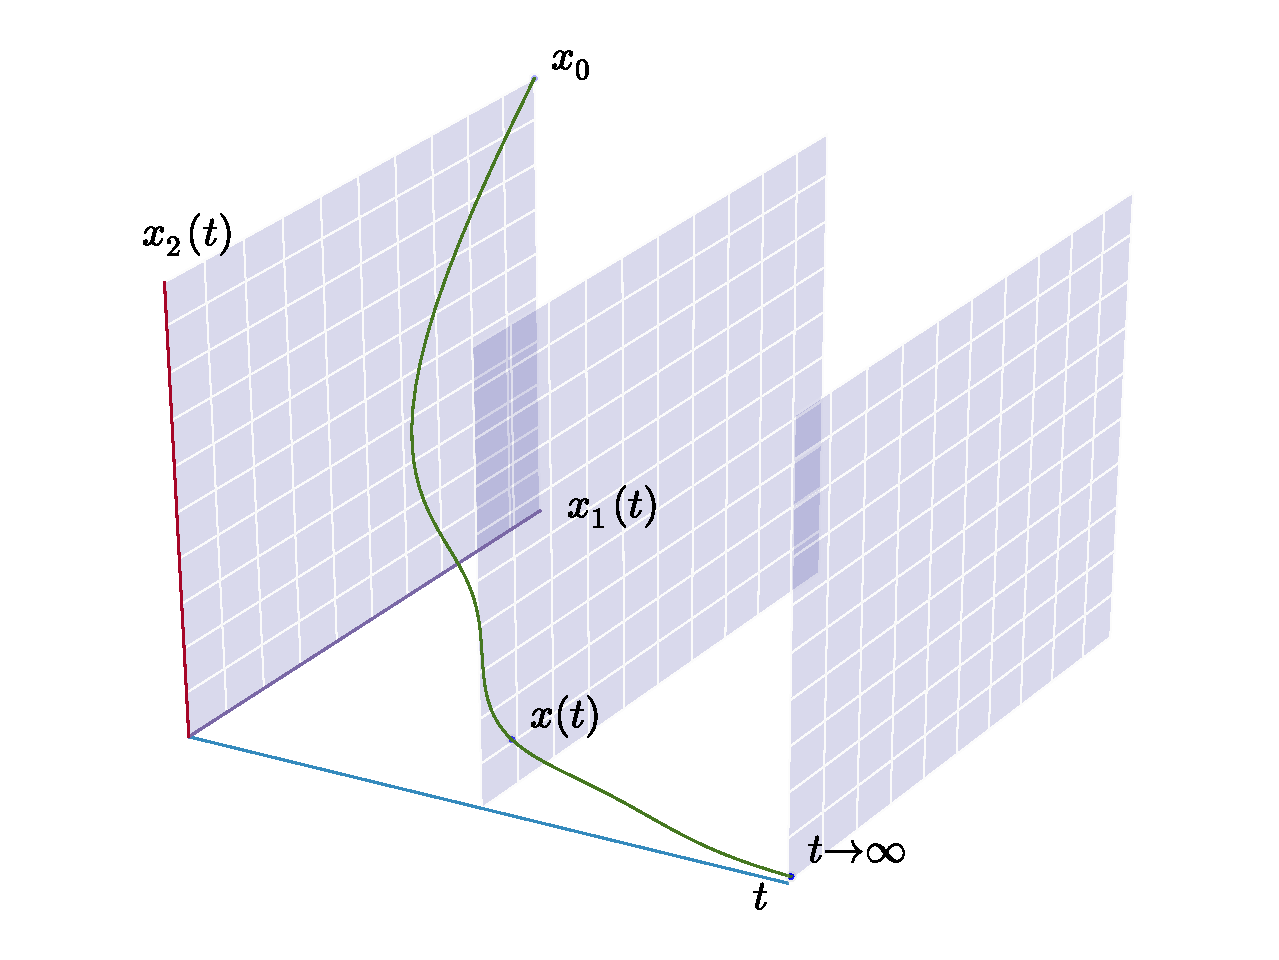
\includegraphics[width=\textwidth]{./imagenes/trayectoria3d.pdf}
        \caption{\label{fig:trayectoriaoptima}Trayectoria óptima solución del sistema.}
    \end{marginfigure}

    Si bien hemos usado a $\lambda$, aun no hemos mencionado que esta variable representa el coestado del sistema y si bien las condiciones de frontera del sistema son correctas, cabe mencionar que lo que realmente queremos es que $x(0) = x_0$ y $\lim_{t \to \infty} x(t) = 0$, por lo que hace falta relacionar al estado del sistema, $x(t)$, con el coestado, $\lambda(t)$.

    En base a la ecuación~\ref{eq:conop4} se propone que la solución sea una realimentación de estado, para esto se propone que el estado $x$ y el coestado $\lambda$ esten relacionados por una matriz $P$, esto es:

    \begin{equation} \label{eq:conop7}
        \lambda = P x
    \end{equation}

    Por lo que de las ecuaciones~\ref{eq:conop6} y~\ref{eq:conop7}, podemos obtener que:

    \begin{equation*}
        \begin{pmatrix}
            I \\
            P
        \end{pmatrix} \dot{x}=
        \begin{pmatrix}
            A & -b \rho^{-1} b^T \\
            - Q & - A^T
        \end{pmatrix}
        \begin{pmatrix}
            I \\
            P
        \end{pmatrix} x
    \end{equation*}

    si premultiplicamos esta expresión con $\begin{pmatrix} P & -I \end{pmatrix}$, obtendremos:

    \begin{equation*}
        0 =
        \begin{pmatrix}
            P A + Q & -P b \rho^{-1} b^T + A^T
        \end{pmatrix}
        \begin{pmatrix}
            I \\
            P
        \end{pmatrix} x
    \end{equation*}

    \begin{equation*}
        0 = \left( A^T P + P A - P b \rho^{-1} b^T P + Q \right) x \quad \forall x \text{ solución del sistema~\ref{eq:conop1}}
    \end{equation*}

    Por lo que hemos llegado a la ecuación algebraica de Riccati:

    \begin{equation} \label{eq:conop8}
        A^T P + P A - P b \rho^{-1} b^T P + Q = 0
    \end{equation}

    siendo la ley de control óptimo (de las ecuaciones~\ref{eq:conop4} y~\ref{eq:conop7}):

    \begin{equation} \label{eq:conop9}
        u = -f_*^T x
    \end{equation}

    donde $f_*^T = \rho^{-1} b^T P$.

    Note que de las ecuaciones~\ref{eq:conop8} y~\ref{eq:conop9}, se obtiene la ecuación de Lyapunov del sistema en lazo cerrado:

    \begin{eqnarray}
        A^T P + P A - P b f_*^T & = & -Q \nonumber \\
        A^T P + P \left( A - b f_*^T \right) & = & - Q \nonumber \\
        \left( A - b f_*^T \right)^T P + P \left( A - b f_*^T \right) & = & - \left( Q + f_* b^T P \right) \nonumber \\
        \left( A - b f_*^T \right)^T P + P \left( A - b f_*^T \right) & = & - \left( Q + f_* \rho f_*^T \right)
    \end{eqnarray}

    En donde la expresión del lado derecho debe ser $\left( Q + f_* b^T P \right) = \left( Q + f_* b^T P \right)^T \ge 0$, por lo que tambien pediremos que $P$ sea simétrica y semidefinida positiva ($P = P^T \ge 0$).

    Como nota final, tan solo hacemos notar que el sistema realimentado queda:

    \begin{equation} \label{eq:conop12}
        \frac{dx}{dt} = (A - b f_*^T) x
    \end{equation}

    Y que una manera de interpretar la minimización del indice de desempeño es con la siguiente gráfica:

    \begin{marginfigure}
        \centering
        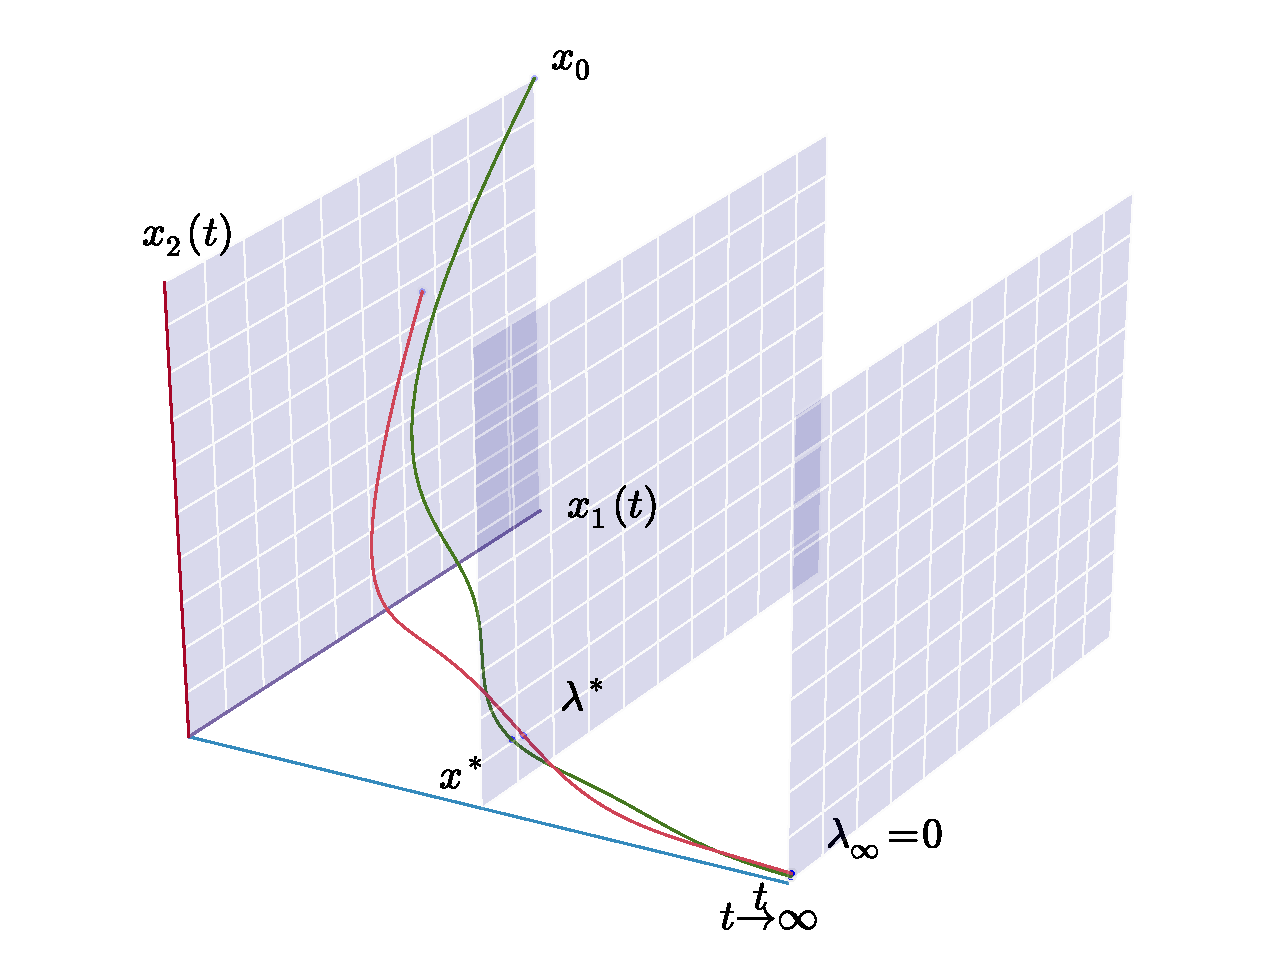
\includegraphics[width=\textwidth]{./imagenes/trayectorias3d.pdf}
        \caption{\label{fig:trayectoriaoptima}Trayectoria óptima solución del sistema del estado y coestado.}
    \end{marginfigure}

%-------------------------------------------------------------------------------
%	EMPIEZA SECCION
%-------------------------------------------------------------------------------

    \newpage
    \section{Propiedades de la matriz de Hamilton}

%-------------------------------------------------------------------------------

        \subsection{La controlabilidad del par $(A, b)$, garantiza la existencia de la solución del problema de control óptimo.}

            Definiendo la siguiente matriz de cambio de base:

            \begin{equation}
                T =
                \begin{pmatrix}
                    I & 0 \\
                    P & I
                \end{pmatrix}, \quad T^{-1} =
                \begin{pmatrix}
                    I & 0 \\
                    -P & I
                \end{pmatrix}
            \end{equation}

            y aplicando este cambio de base, la representación de estado de la ecuación~\ref{eq:conop6} queda:

            \begin{equation} \label{eq:conop10}
                \begin{pmatrix}
                    \dot{x} \\
                    \dot{\bar{\lambda}}
                \end{pmatrix} =
                \begin{pmatrix}
                    A - b f_*^T & -b \rho^{-1} b^T \\
                    -0 & - (A - b f_*^T)^T
                \end{pmatrix}
                \begin{pmatrix}
                    x \\
                    \bar{\lambda}
                \end{pmatrix}
            \end{equation}

            En efecto:

            \begin{equation*}
                \begin{pmatrix}
                    x \\
                    \bar{\lambda}
                \end{pmatrix} =
                \begin{pmatrix}
                    I & 0 \\
                    -P & I
                \end{pmatrix}
                \begin{pmatrix}
                    x \\
                    \lambda
                \end{pmatrix}
            \end{equation*}

            \begin{eqnarray*}
                T^{-1} M T & = &
                \begin{pmatrix}
                    I & 0 \\
                    -P & I
                \end{pmatrix}
                \begin{pmatrix}
                    A & -b \rho^{-1} b^T \\
                    -Q & P b \rho^{-1} b^T - A^T
                \end{pmatrix}
                \begin{pmatrix}
                    I & 0 \\
                    P & I
                \end{pmatrix} \\
                & = &
                \begin{pmatrix}
                    A & -b \rho^{-1} b^T \\
                    -(PA + Q) & P b \rho^{-1} b^T - A^T
                \end{pmatrix}
                \begin{pmatrix}
                    I & 0 \\
                    P & I
                \end{pmatrix} \\
                & = &
                \begin{pmatrix}
                    A - b \rho^{-1} b^T P & -b \rho^{-1} b^T \\
                    -(A^TP + PA - Pb \rho^{-1} b^T P + Q) & - (A^T + P b \rho^{-1} b^T)
                \end{pmatrix}
            \end{eqnarray*}

            si sustituimos las ecuaciones~\ref{eq:conop8} y~\ref{eq:conop9}, tendremos:

            \begin{equation*}
                T^{-1} M T =
                \begin{pmatrix}
                    A - b f_*^T & - b \rho^{-1} b^T \\
                    0 & -(A - b f_*^T)^T
                \end{pmatrix}
            \end{equation*}

            \begin{nota}
                Note que el determinante de la matrix Hamiltoniana es igual al de esta matriz:

                \begin{eqnarray*}
                    \det{(sI - M)} & = & \det{(sI - T^{-1}MT)} \\
                     & = & (-1)^n \pi(s) \pi(-s)
                \end{eqnarray*}

                donde $\pi(s) = \det{(sI - (A - b f_*^T))}$, es decir que los valores propios de $M$ son simetricos con respecto al eje $j\omega$.
            \end{nota}

            Resolviendo el sistema de la ecuación~\ref{eq:conop10} en el horizonte de tiempo $[0, T]$ y con $A_{f_*} = A - b f_*^T$:

            \begin{eqnarray}
                \bar{\lambda}(t) & = & \exp{(A_{f_*}^T (T - t))} \bar{\lambda}(t) \\
                x(t) & = & \exp{(A_{f_*} t)} x_0 - \int_0^t \exp{(A_{f_*}(t - \tau))} b \rho^{-1} b^T \bar{\lambda}(\tau) d\tau \nonumber
            \end{eqnarray}

            especificamente para nuestro tiempo $T$ y sustituyendo $\bar{\lambda}(t)$ en $x(t)$:

            \begin{equation*}
                x(T) = \exp{(A_{f_*} T)} x_0 - \int_0^T \exp{(A_{f_*}(T - \tau))} b \rho^{-1} b^T \exp{(A_{f_*}^T (T - \tau))} \bar{\lambda}(T) d\tau \bar{\lambda}(T)
            \end{equation*}

            Siendo la parte integral de esta solución el Gramiano de controlabilidad.

            Recordemos que:

            \begin{eqnarray*}
                (A, b) \text{controlable} & \implies & (A_{f_*}, b) \text{controlable} \\
                & \implies & \det{\int_0^T \exp{(A_{f_*}(T - \tau))} b b^T \exp{(A_{f_*}^T (T - \tau))} \bar{\lambda}(T) d\tau} \\
                & \implies & \det{\int_0^T \exp{(A_{f_*}(T - \tau))} b \rho^{-1} b^T \exp{(A_{f_*}^T (T - \tau))} \bar{\lambda}(T) d\tau \bar{\lambda}(T)}
            \end{eqnarray*}

            Asi pues, asumiremos la controlabilidad del par $(A, b)$.

            Sea $x^*$ la trayectoria óptima, por lo que:

            \begin{equation*}
                J(x^*, x_0) \le J(x, x_0)
            \end{equation*}

            para toda solución de la ecuación~\ref{eq:conop1}.

            Entonces, el coestado $\bar{\lambda}^*$ que minimice a $Ja$ será:

            \begin{equation*}
                Ja(x^*, \lambda^*, x_0, \bar{\lambda}(T)) \le Ja(x, \bar{\lambda}, x_0, \bar{\lambda}(T))
            \end{equation*}

            para todo par $(x, \bar{\lambda})$ solución de la ecuación~\ref{eq:conop10} y estará caracterizada por:

            \begin{eqnarray*}
                \bar{\lambda}^*(T) & = & W_c^{-1}(0, T) \left( \exp{(A_{f_*} T)} x_0 - x^*(T) \right) \\
                W_c (0, T) & = & \int_0^T \exp{\left( A_{f_*}(T-\tau) \right)} b \rho^{-1} b^T \exp{\left( A_{f_*}^T(T-\tau) \right)} d\tau
            \end{eqnarray*}

            por lo que si $W_c$ es invertible, existe una solución; y para que $W_c$ sea invertible, el par $(A, b)$ debe ser controlable.

%-------------------------------------------------------------------------------

        \subsection{La observabilidad del par $(Q_{\sfrac{1}{2} ,A})$, donde $Q = Q_{\sfrac{1}{2}}^T Q_{\sfrac{1}{2}}$ , asegura la solución estable de la solución de Riccati.}

        De las ecuaciones~\ref{eq:conop8} y~\ref{eq:conop9}, la ecuación de Riccati se puede escribir de la siguiente manera:

        \begin{eqnarray*}
            A^T P + P A - P b \rho^{-1} b^T P & = & -Q \\
            (A - b f_{*}^T) P + P (A - b f_{*}^T) & = & -Q - f_{*} b^T P \\
            A_{f_*}^T P + P A_{f_*} & = & -Q - f_* \rho f_*^T
        \end{eqnarray*}

        en donde el termino izquierdo se reconoce de la ecuación de Lyapunov y el termino derecho sabemos que es una matriz simétrica, por lo que se obtiene la siguiente ecuación de Lyapunov:

        \begin{equation} \label{eq:conop11}
            A_{f_*}^T P + P A_{f_*} =
            \begin{pmatrix}
                -Q_{\sfrac{1}{2}}^T & f_*
            \end{pmatrix}
            \begin{pmatrix}
                I & 0 \\
                0 & \rho
            \end{pmatrix}
            \begin{pmatrix}
                Q_{\sfrac{1}{2}} \\
                f_*^T
            \end{pmatrix}
        \end{equation}

        en donde podemos nombrar al segundo termino como:

        \begin{equation*}
            \bar{Q} =
            \begin{pmatrix}
                -Q_{\sfrac{1}{2}}^T & f_*
            \end{pmatrix}
            \begin{pmatrix}
                I & 0 \\
                0 & \rho
            \end{pmatrix}
            \begin{pmatrix}
                Q_{\sfrac{1}{2}} \\
                f_*^T
            \end{pmatrix}
        \end{equation*}

        y de donde tenemos que $P = P^T > 0$ y $\bar{Q} = \bar{Q}^T \ge 0$.

        Si recordamos el corolario~\ref{co:lyap1} de Kalman, sabemos que podemos escoger una $Q \ge 0$ para la ecuación de Lyapunov, siempre y cuando el par $(Q_{\sfrac{1}{2}}, A)$ sea observable.

        Notemos que la observabilidad del par $(Q_{\sfrac{1}{2}}, A)$, implica la observabilidad del par $\left( \begin{pmatrix} Q_{\sfrac{1}{2}} \\ f_*^T \end{pmatrix} , A_{f_*} \right)$.

        En efecto, primero notamos que:

        \begin{equation}
            \begin{pmatrix}
                I & 0 & 0 \\
                0 & -b & I \\
                0 & 1 & 0
            \end{pmatrix}
            \begin{pmatrix}
                Q_{\sfrac{1}{2}} \\
                f_*^T \\
                sI - A + b f_*^T
            \end{pmatrix} =
            \begin{pmatrix}
                Q_{\sfrac{1}{2}} \\
                sI - A \\
                f_*^T
            \end{pmatrix}
        \end{equation}

        lo cual implica que:

        \begin{equation*}
            \rango{\begin{pmatrix} Q_{\sfrac{1}{2}} \\ sI - A \end{pmatrix}} \le \rango{\begin{pmatrix} Q_{\sfrac{1}{2}} \\ sI - A \\ f_*^T \end{pmatrix}}
        \end{equation*}

        es decir, aumentar filas en una matriz no disminuye el rango, y de la ecuación~\ref{eq:conop11} podemos notar que:

        \begin{equation}
            \rango{\begin{pmatrix} Q_{\sfrac{1}{2}} \\ f_*^T \\ sI - A + b f_*^T \end{pmatrix}} = \rango{\begin{pmatrix} Q_{\sfrac{1}{2}} \\ sI - A \\ f_*^T \end{pmatrix}} \le n
        \end{equation}

        por lo que:

        \begin{equation}
            \rango{\begin{pmatrix} Q_{\sfrac{1}{2}} \\ sI - A \end{pmatrix}} = n \forall s \in \mathbb{C} \implies \rango{\begin{pmatrix} Q_{\sfrac{1}{2}} \\ f_*^T \\ sI - A + b f_*^T \end{pmatrix}} = n \forall s \in \mathbb{C}
        \end{equation}

        \begin{nota}
            Criterio del rango de Popov-Belevitch-Hautus
            \begin{enumerate}[i]
                \item El par $(A, b)$ es controlable si y solo si:

                \begin{equation*}
                    \rango{\begin{pmatrix} sI - A & b \end{pmatrix}} = n \quad \forall s \in \mathbb{C}
                \end{equation*}

                \item El par $(c^T, A)$ es observable si y solo si:

                \begin{equation*}
                    \rango{\begin{pmatrix} c^T & sI - A \end{pmatrix}} = n \quad \forall s \in \mathbb{C}
                \end{equation*}
            \end{enumerate}
        \end{nota}

        Tomando en cuenta el criterio de Popov-Belevitch-Hautus podemos afirmar que si el par $\left( \begin{pmatrix} Q_{\sfrac{1}{2}} \\ f_*^T \end{pmatrix} , sI - A_{f_*} \right)$ es observable, tambien lo será $\left( \begin{pmatrix} Q_{\sfrac{1}{2}} \\ f_*^T \end{pmatrix} , A_{f_*} \right)$ y por lo tanto tambien lo será $\left( Q_{\sfrac{1}{2}} , A_{f_*} \right)$, es decir:

        \begin{equation*}
            (Q_{\sfrac{1}{2}}, A) \text{ es observable } \implies \left( \begin{pmatrix}Q_{\sfrac{1}{2}} \\ f_*^T \end{pmatrix}, A \right) \text{ es observable }
        \end{equation*}

        Construyamos entonces la siguiente función de Lyapunov:

        \begin{equation}
            V(x(t)) = x^T(t) P x(t)
        \end{equation}

        derivando la función de Lyapunov a lo largo de las trayectorias solución de la ecuación~\ref{eq:conop12} y sustituyendo la ecuación~\ref{eq:conop11} tendremos:

        \begin{eqnarray*}
            \frac{dV(x(t))}{dt} & = & x^T(t)(A_{f_*}^T P + P A_{f_*})x(t) \\
             & = & -x^T(t) \bar{Q} x(t)
        \end{eqnarray*}

        por lo que el criterio de estabilidad de Kalman se deduce la estabilidad Hurwitz del sistema en lazo cerrado, ademas la solución es única, debido al corolario~\ref{co:lyap2}.
